%%%%%%%%%%%%%%%%%%%%%%%%%%%%%%%%%%%%%%%%%
% Beamer Presentation
% LaTeX Template
% Version 1.0 (10/11/12)
%
% This template has been downloaded from:
% http://www.LaTeXTemplates.com
%
% License:
% CC BY-NC-SA 3.0 (http://creativecommons.org/licenses/by-nc-sa/3.0/)
%
%%%%%%%%%%%%%%%%%%%%%%%%%%%%%%%%%%%%%%%%%

%----------------------------------------------------------------------------------------
%	PACKAGES AND THEMES
%----------------------------------------------------------------------------------------

\documentclass[9pt]{beamer}

\mode<presentation> {

% The Beamer class comes with a number of default slide themes
% which change the colors and layouts of slides. Below this is a list
% of all the themes, uncomment each in turn to see what they look like.

%\usetheme{default}
%\usetheme{AnnArbor}
%\usetheme{Antibes}
%\usetheme{Bergen}
%\usetheme{Berkeley}
%\usetheme{Berlin}
%\usetheme{Boadilla}
%\usetheme{CambridgeUS}
%\usetheme{Copenhagen}
%\usetheme{Darmstadt}
%\usetheme{Dresden}
%\usetheme{Frankfurt}
%\usetheme{Goettingen}
%\usetheme{Hannover}
%\usetheme{Ilmenau}
%\usetheme{JuanLesPins}
%\usetheme{Luebeck}
\usetheme{Madrid}
%\usetheme{Malmoe}
%\usetheme{Marburg}
%\usetheme{Montpellier}
%\usetheme{PaloAlto}
%\usetheme{Pittsburgh}
%\usetheme{Rochester}
%\usetheme{Singapore}
%\usetheme{Szeged}
%\usetheme{Warsaw}

% As well as themes, the Beamer class has a number of color themes
% for any slide theme. Uncomment each of these in turn to see how it
% changes the colors of your current slide theme.

%\usecolortheme{albatross}
%\usecolortheme{beaver}
%\usecolortheme{beetle}
%\usecolortheme{crane}
%\usecolortheme{dolphin}
%\usecolortheme{dove}
%\usecolortheme{fly}
%\usecolortheme{lily}
%\usecolortheme{orchid}
%\usecolortheme{rose}
%\usecolortheme{seagull}
%\usecolortheme{seahorse}
%\usecolortheme{whale}
%\usecolortheme{wolverine}

%\setbeamertemplate{footline} % To remove the footer line in all slides uncomment this line
%\setbeamertemplate{footline}[page number] % To replace the footer line in all slides with a simple slide count uncomment this line

%\setbeamertemplate{navigation symbols}{} % To remove the navigation symbols from the bottom of all slides uncomment this line
}
\usepackage{bm}
\usepackage{upgreek}
\usepackage[backend=bibtex,sorting=none]{biblatex}
\usepackage{graphicx} % Allows including images
\usepackage{booktabs} % Allows the use of \toprule, \midrule and \bottomrule in tables
\setbeamerfont{caption}{size=\tiny}
\setbeamerfont{footnote}{size=\tiny}
\setbeamerfont{frametitle}{size=\huge}
\setbeamerfont{title}{size=\huge}
\addbibresource{slides.bib} %BibTeX数据文件及位置
\def\mathfamilydefault{\rmdefault}
%----------------------------------------------------------------------------------------
%	TITLE PAGE
%----------------------------------------------------------------------------------------

\title[RIS-assisted RadCom]{RIS-Assisted\\
Joint Radar and Communications\\
Beamforming Design} % The short title appears at the bottom of every slide, the full title is only on the title page

\author{Zhaolin Wang} % Your name
\institute[Imperial] % Your institution as it will appear on the bottom of every slide, may be shorthand to save space
{
Communications and Signal Processing Group\\ % Your institution for the title page
Department of Electrical and Electronic Engineering\\
Imperial College London
\medskip
}
\date{March 3, 2021} % Date, can be changed to a custom date

\begin{document}

\begin{frame}
\titlepage % Print the title page as the first slide
\end{frame}

%------------------------------------------------

\begin{frame}
\frametitle{Communication and Radar Spectrum Sharing}
\begin{itemize}
  \item \textbf{Motivation} \footfullcite{8999605}
    \begin{itemize}
      \item Radar systems utilize numerous spectrum bands below 10 GHz, leading to sever spectrum congestion with future wireless communications systems.
    \end{itemize}
  \item \textbf{Communication and Radar Spectrum Sharing (CRSS)} \footfullcite{9201513}
    \begin{itemize}
      \item Coexistence of existing radar and communications.
      \item Co-design for dual-functional radar and communications (DFRC)
        \begin{enumerate}
          \item Radar-centric (information embedding)
          \item Communication-centric (joint beamforming design)
        \end{enumerate}
    \end{itemize}
\end{itemize}
\begin{figure}
  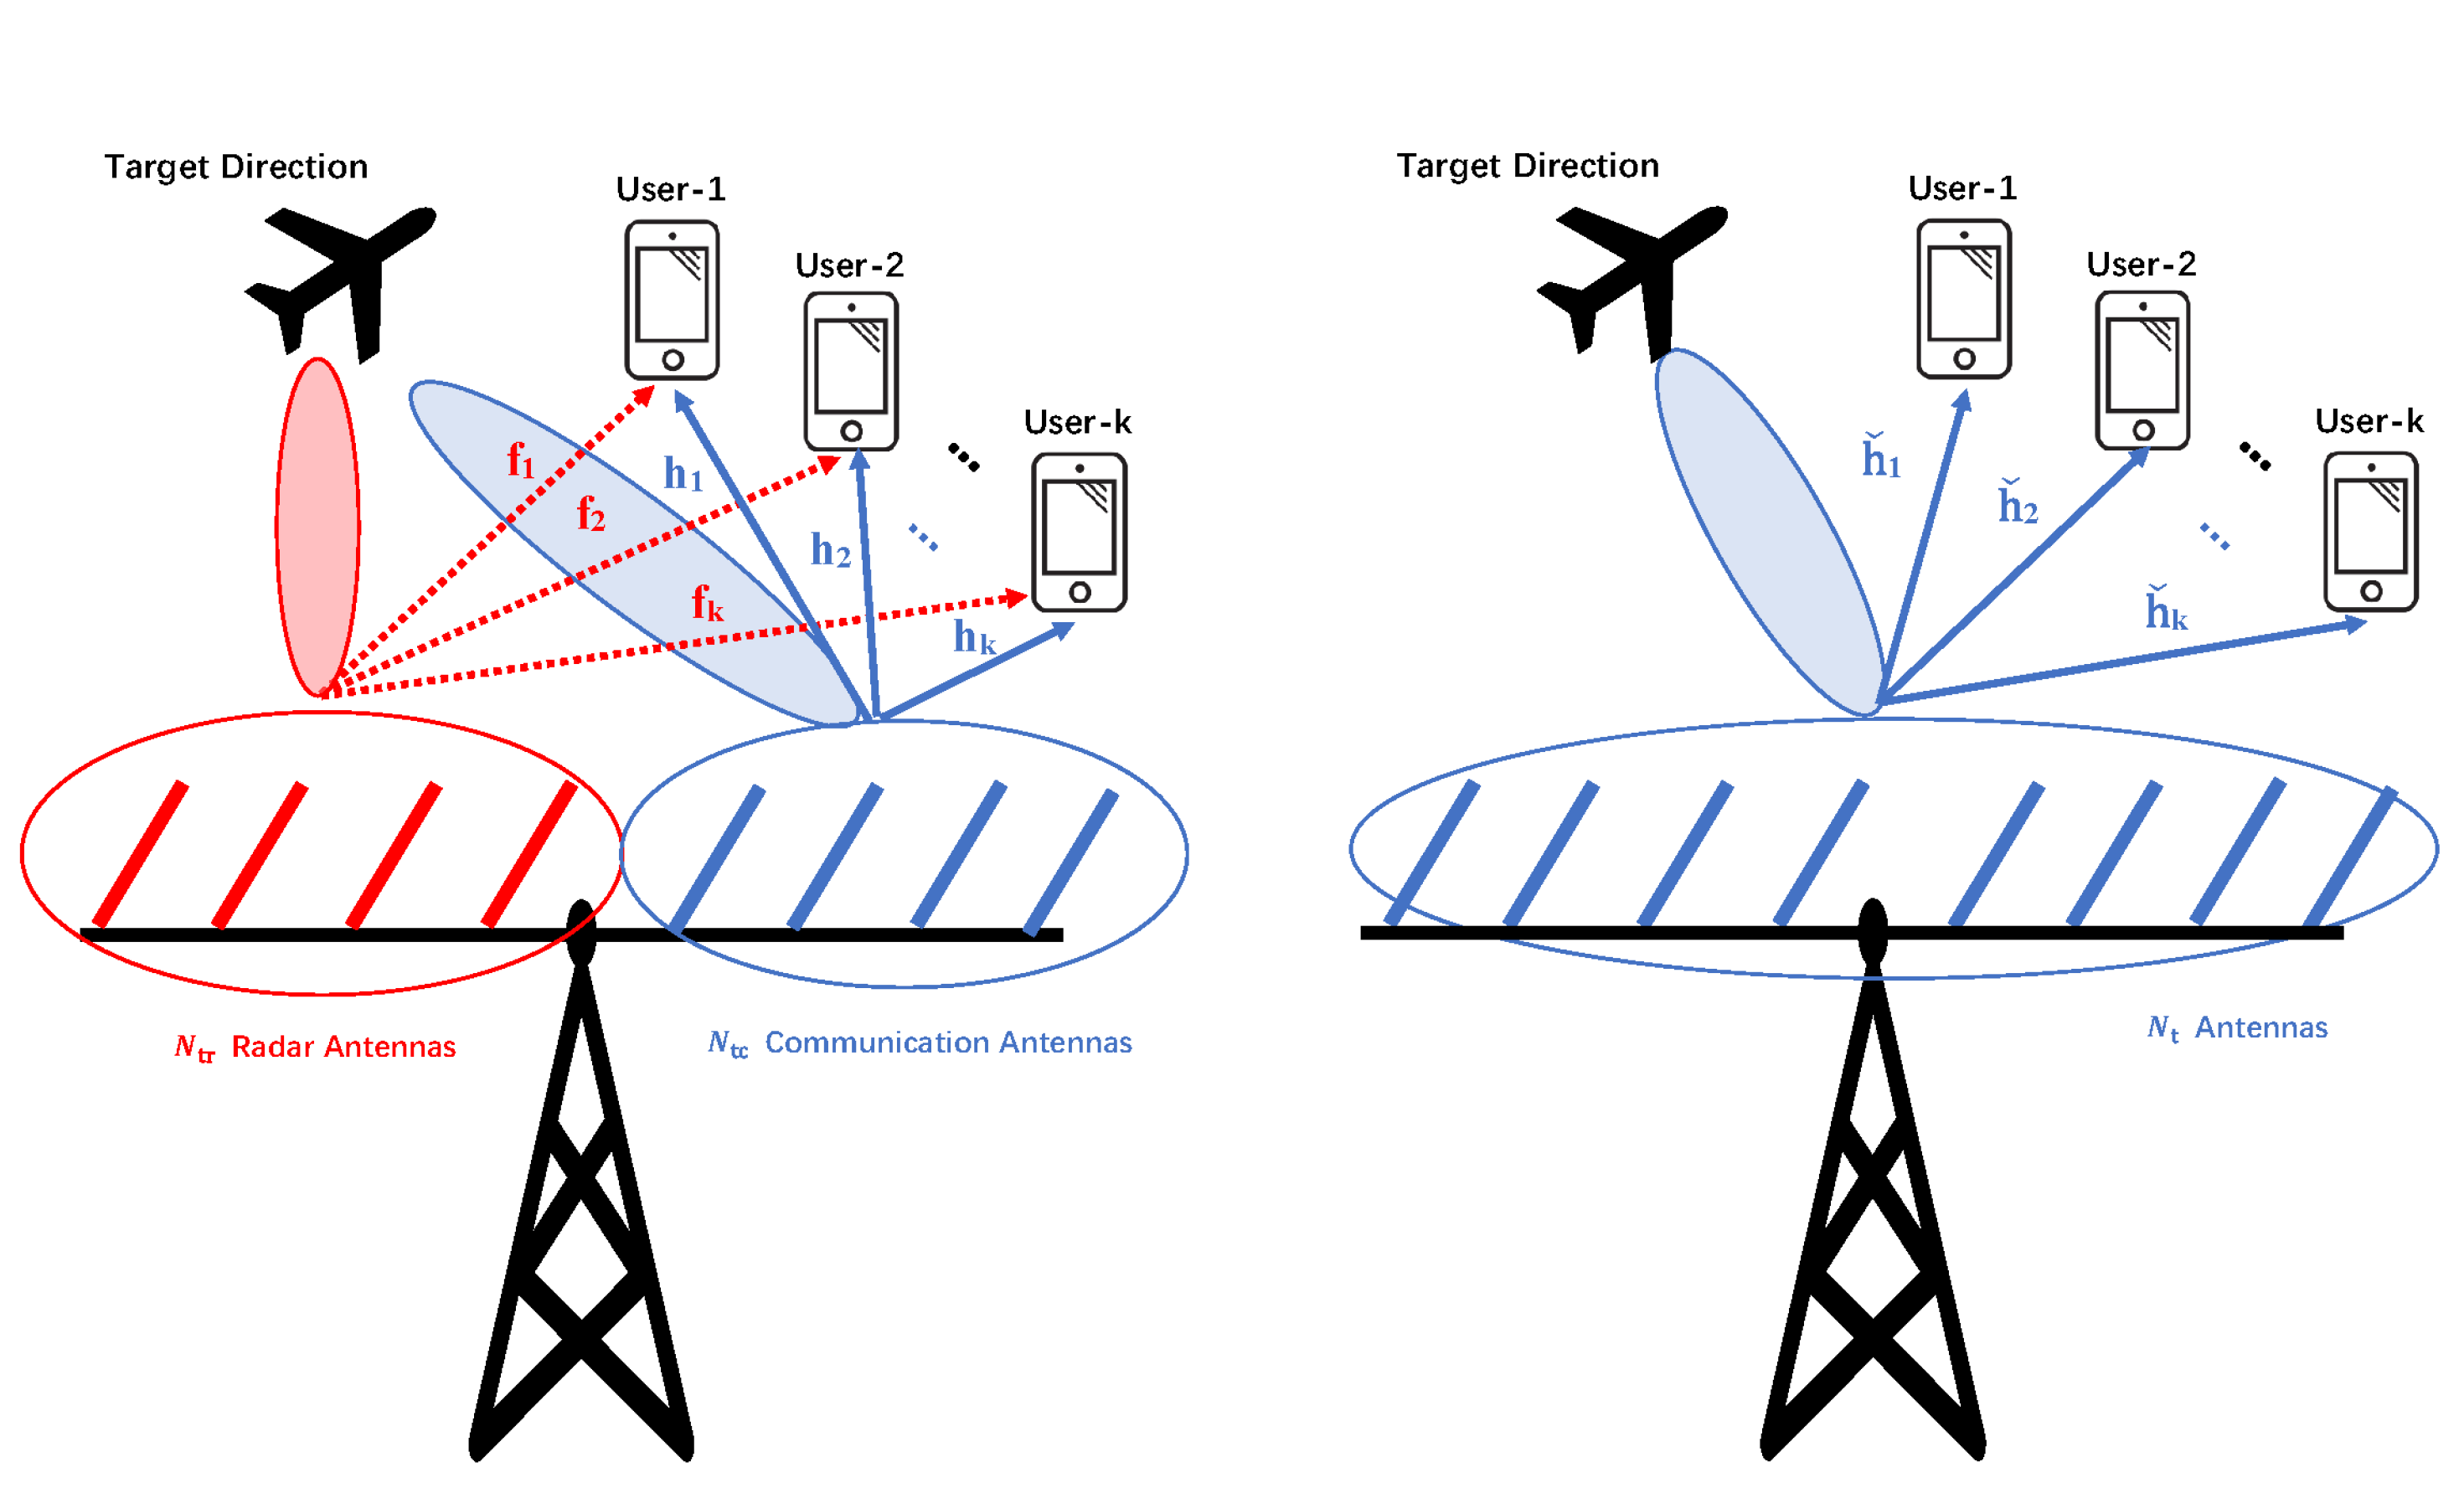
\includegraphics[width=0.4\linewidth]{Fig1.png}
  \caption{Schematic diagram for separated and shared multi-antenna
  joint RadCom \footfullcite{9200993}}
\end{figure}
\end{frame}

%------------------------------------------------

\begin{frame}
\frametitle{Trade-off between Radar and Communication}

\begin{columns}[c]
\column{.65\textwidth}
\begin{align*}
  \max_{\mathbf{P},\mathbf{R}_x} \rho&\sum_{k=1}^K \mu_k R_k(\mathbf{P},\mathbf{R}_x) + \\
  &\mathbf{a}_1^H(\varphi_m)\mathbf{R}_x \mathbf{a}_1(\varphi_m) + \mathbf{a}_2^H(\varphi_m)\mathbf{P}\mathbf{P}^H\mathbf{a}_2(\varphi_m)\\
  \mathbf{s.t.} \quad  &\mathrm{diag}(\mathbf{R}_x) = \frac{P_r \mathbf{1}^{M_r \times 1}}{M_r} \\ 
  &\mathrm{Tr} (\mathbf{P}\mathbf{P}^H) \leq P_c \\
  &\mathbf{R}_x \succeq 0 
\end{align*}

\column{.35\textwidth}
\begin{figure}
  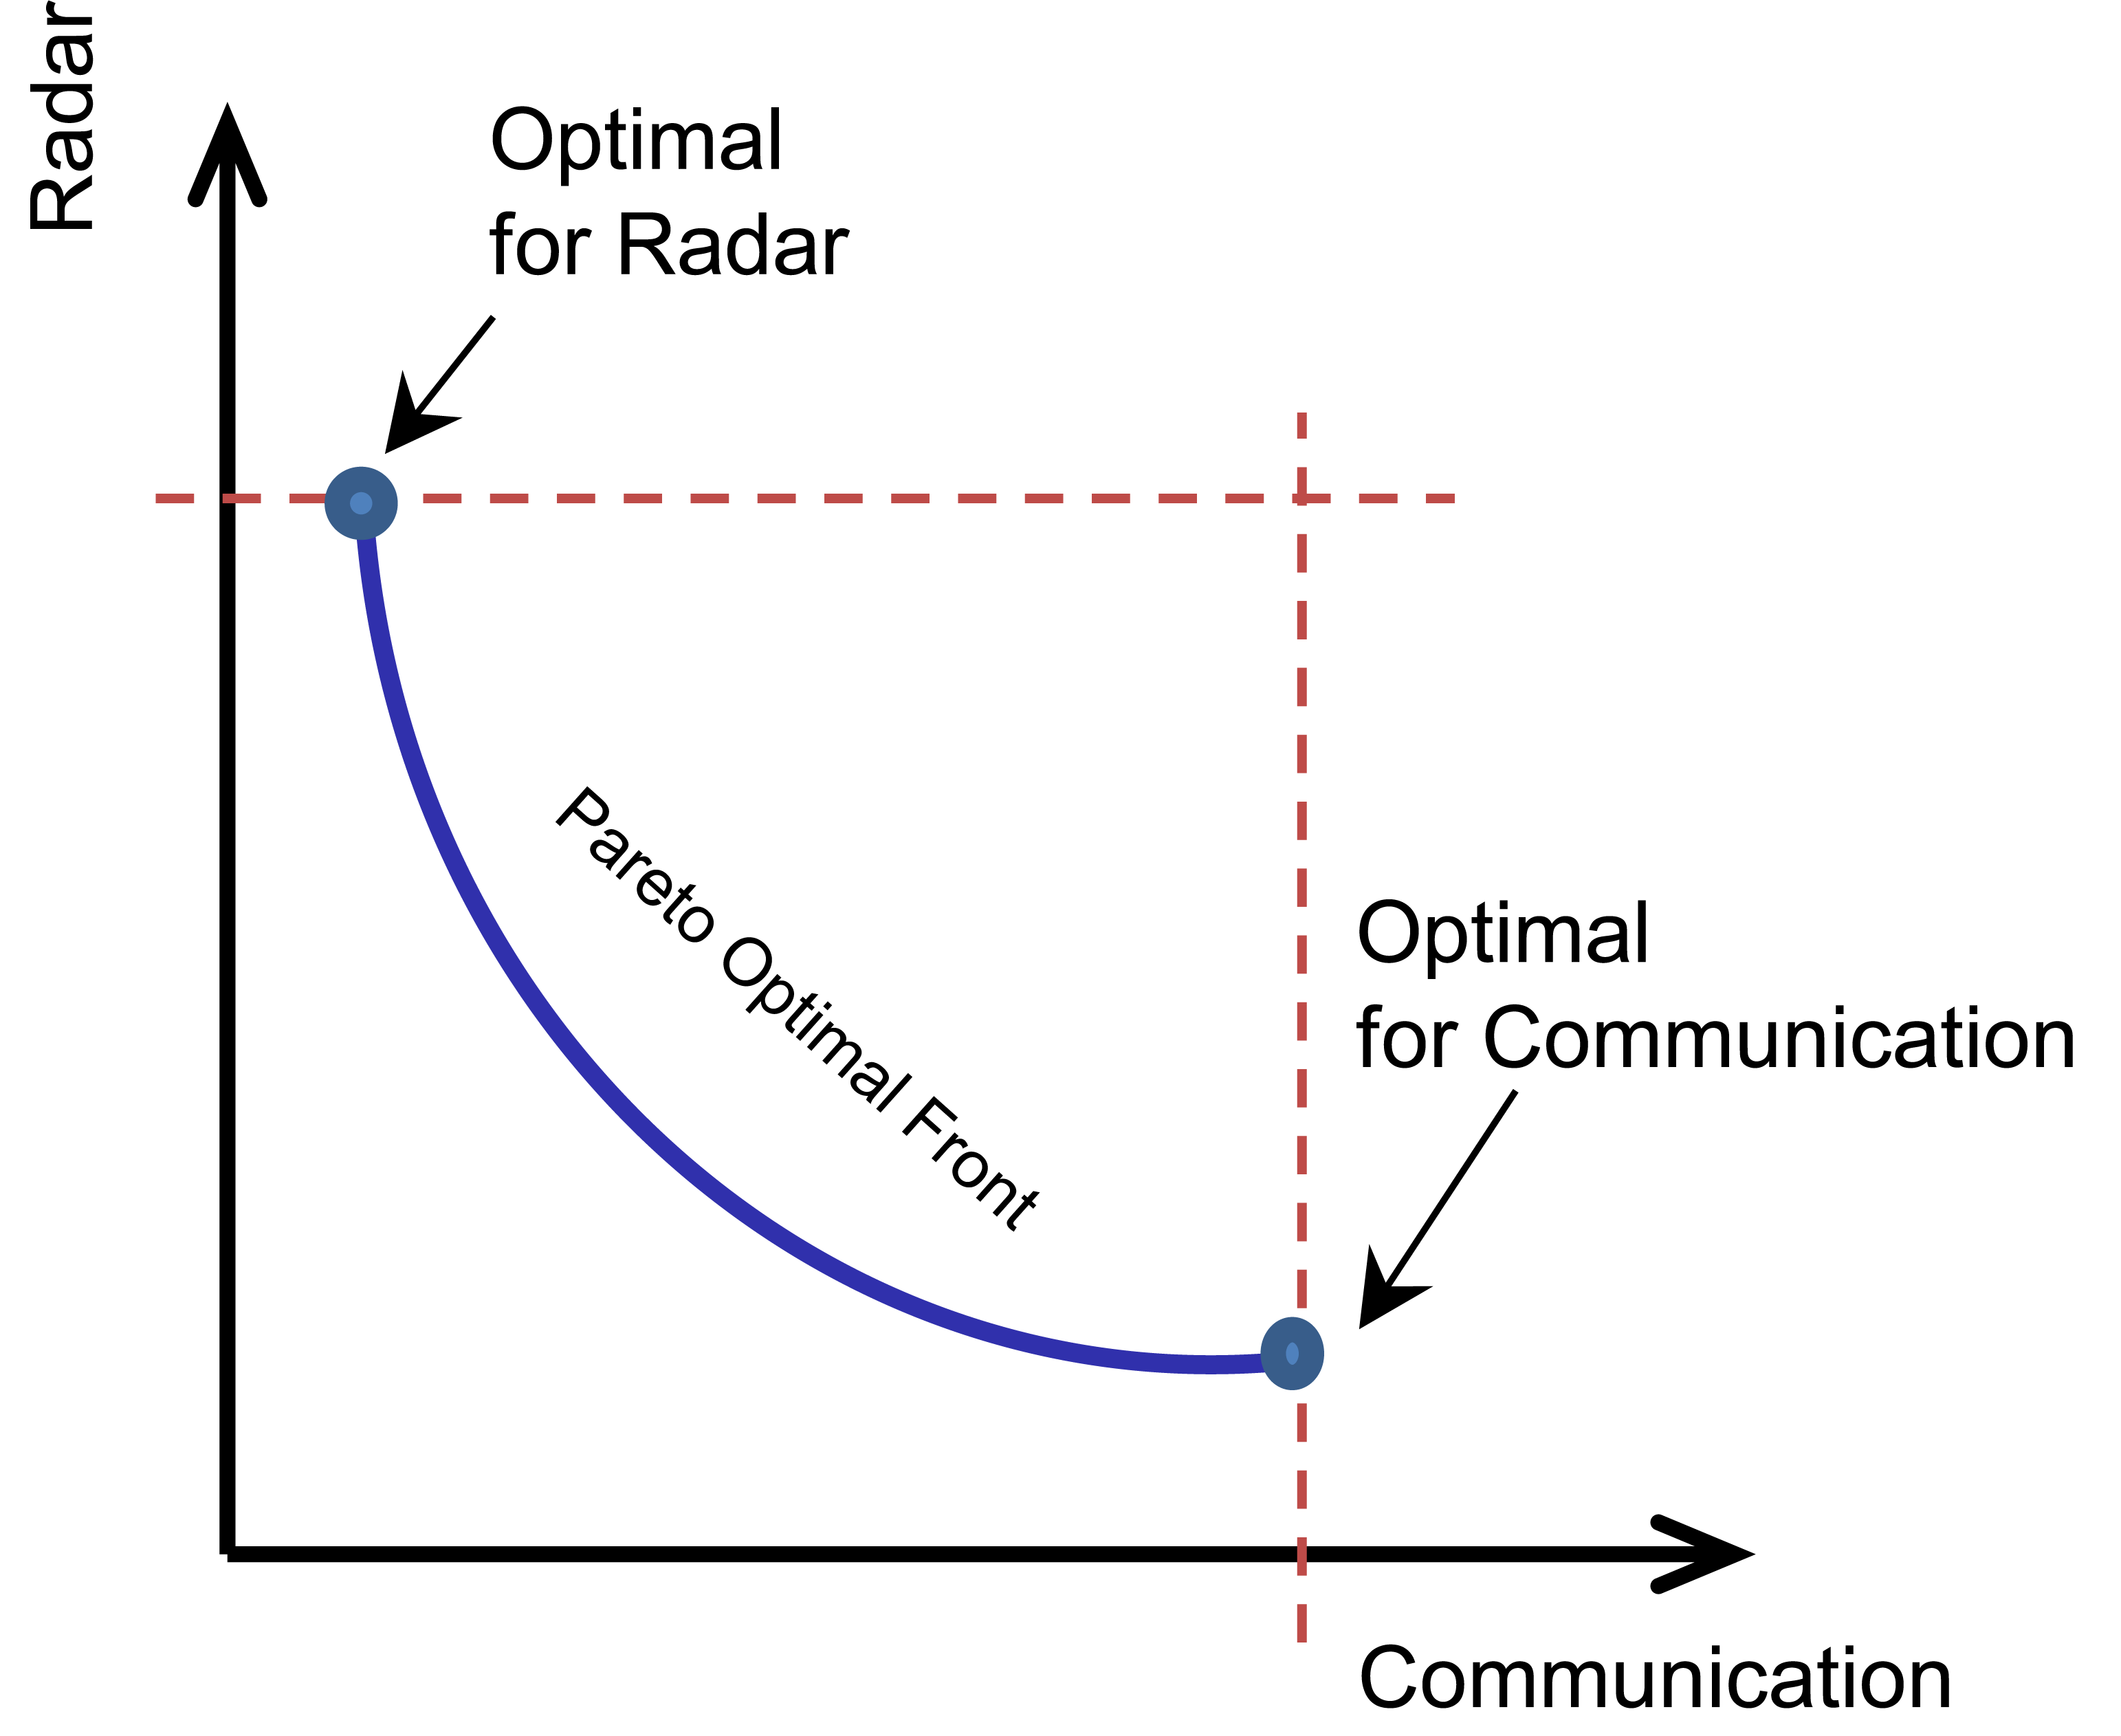
\includegraphics[width=0.9\linewidth]{Fig2.png}
  \caption{Pareto Optimal Front}
\end{figure}
\end{columns}

\begin{itemize}
  \item What if the channel is totally controllable?
  \begin{itemize}
    \item Precoder (beamforming) is only for Radar
    \item Control the channel to meet the Communication requirement
  \end{itemize}

  \item Reconfigurable Intelligent Surface (RIS) \footfullcite{liu2020reconfigurable}
  \begin{itemize}
    \item Composed of many small and low-cost reflecting elements
    \item Achieve the desired propagation characteristics 
  \end{itemize}
\end{itemize}
\end{frame}

%------------------------------------------------

\begin{frame}
  \frametitle{RIS-Assisted Joint RadCom Beamforming Design}
  \begin{itemize}
    \item System Model
      \begin{itemize}
        \item $M_r$ antennas for the radar, $M_c$ antennas for the communication
        \item $N$ reflecting elements at RIS
        \item $K$ users with single antenna; 1 target
        \item Observation at user $k$
          \begin{equation*}
            y_k = \mathbf{h}_k^H \mathbf{\Theta}^H \mathbf{H}_c \sum_{k=1}^K \mathbf{p}_j s_j + \mathbf{h}_k^H \mathbf{\Theta}^H \mathbf{H}_r \mathbf{r} + n_k
          \end{equation*}
        \item SINR and Achievable Rate at user $k$
          \begin{align*}
            &\gamma_k(\mathbf{P},\mathbf{R}_x,\mathbf{\Theta}) = \frac{|\mathbf{h}_k^H \mathbf{\Theta}^H \mathbf{H}_c \mathbf{p}_k|^2} {\sum_{j=1,j\neq k}^{K} |\mathbf{h}_k^H \mathbf{\Theta}^H \mathbf{H}_c \mathbf{p}_j|^2 + \mathbf{f}_k^H \mathbf{R}_x \mathbf{f}_k + 1}\\
            &R_k(\mathbf{P},\mathbf{R}_x,\mathbf{\Theta}) = \log_2 ( 1 + \gamma_k (\mathbf{P},\mathbf{R}_x,\mathbf{\Theta}))
          \end{align*}
      \end{itemize}
  \end{itemize}


  \begin{figure}
    \centering
    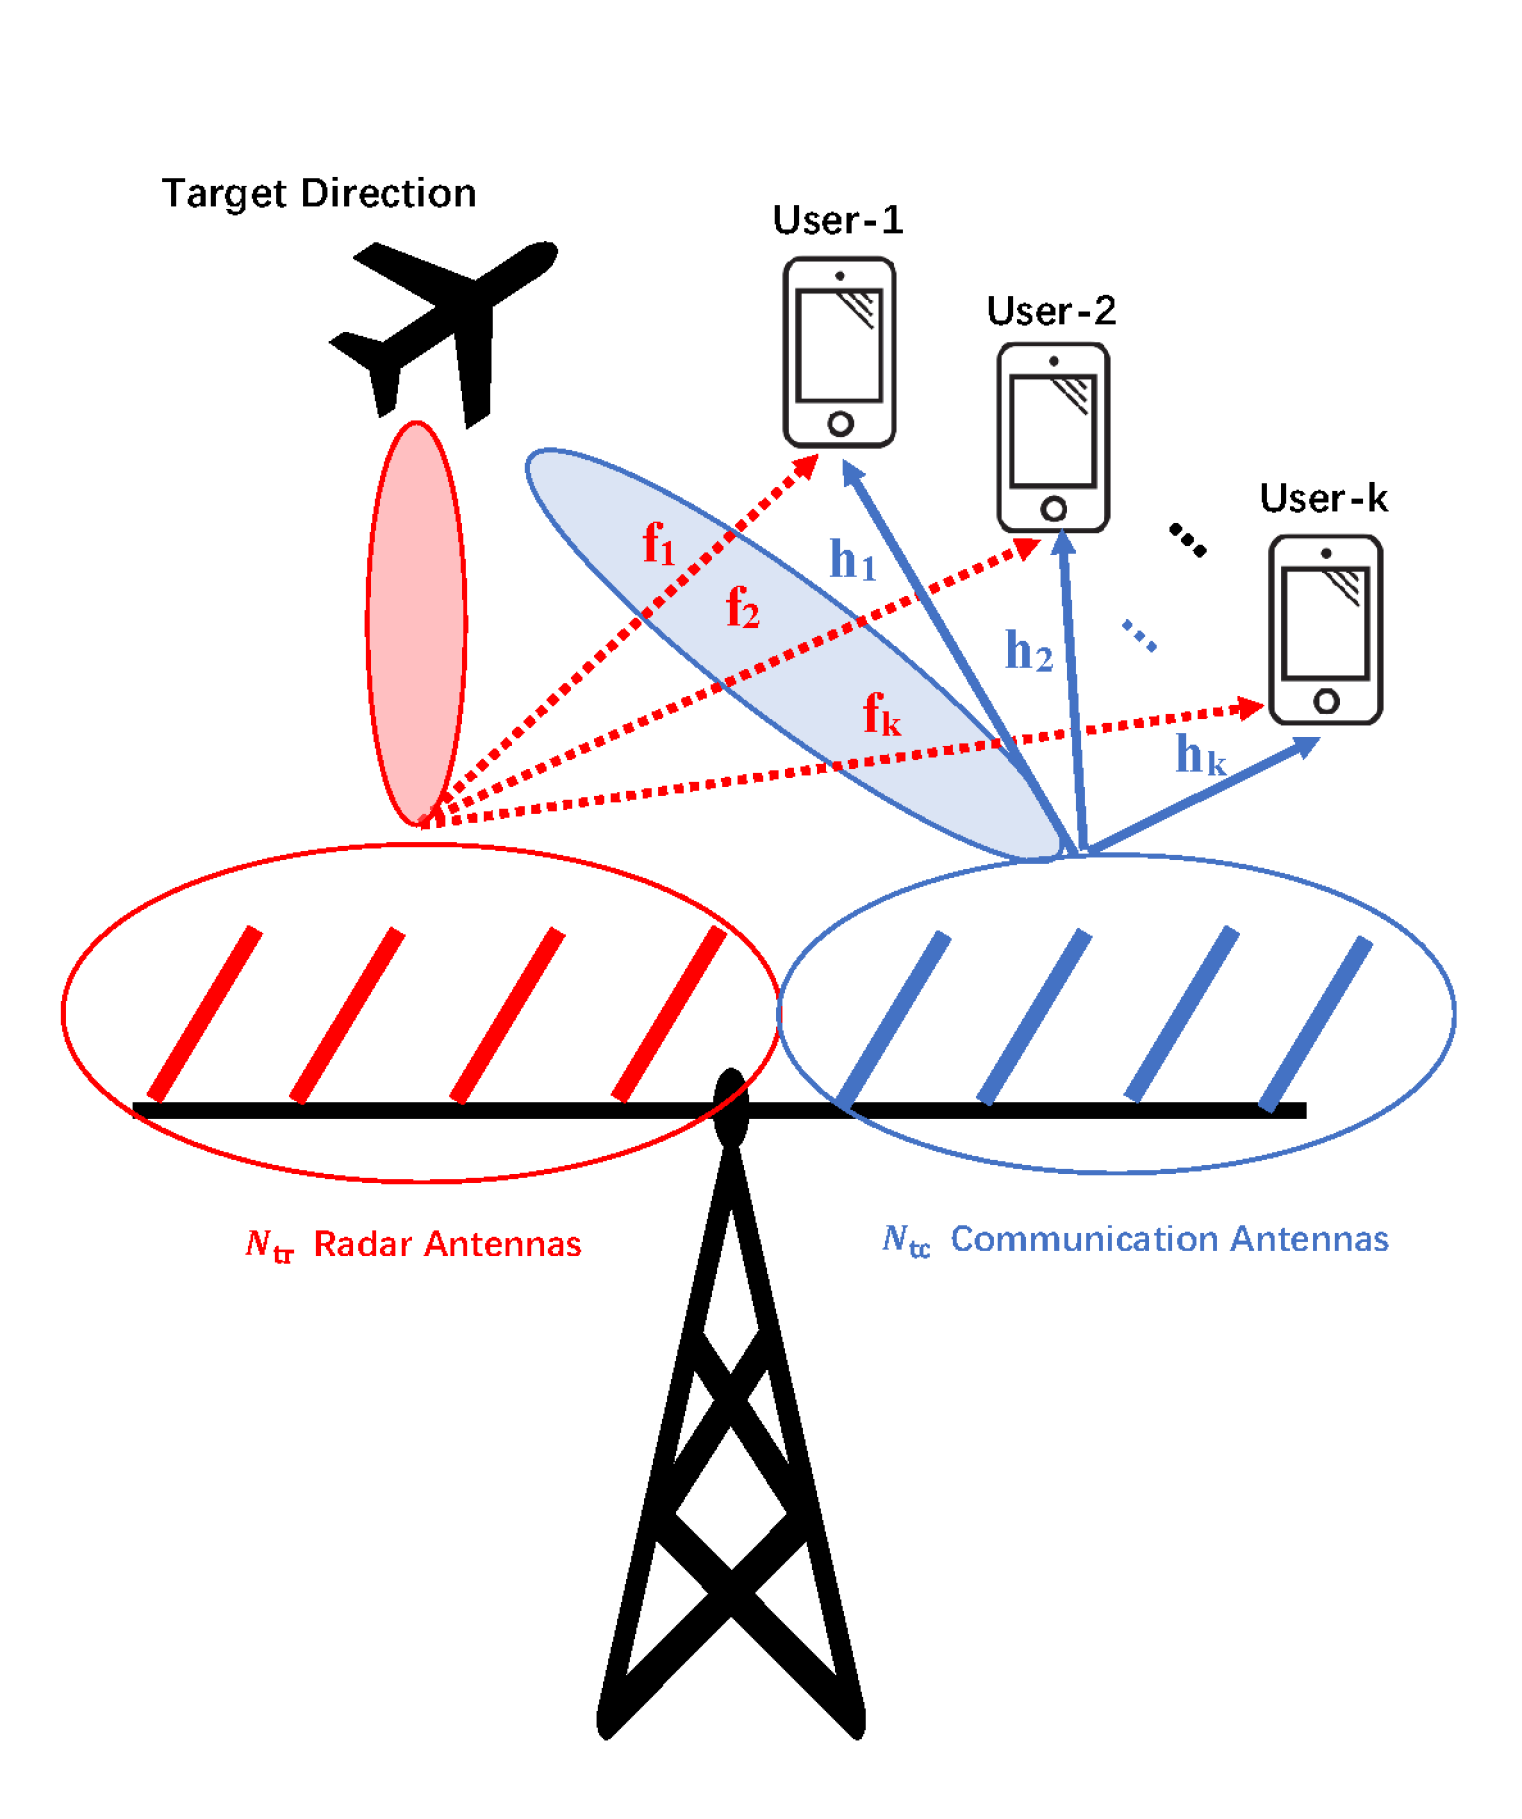
\includegraphics[totalheight=3cm]{Fig3.png}
    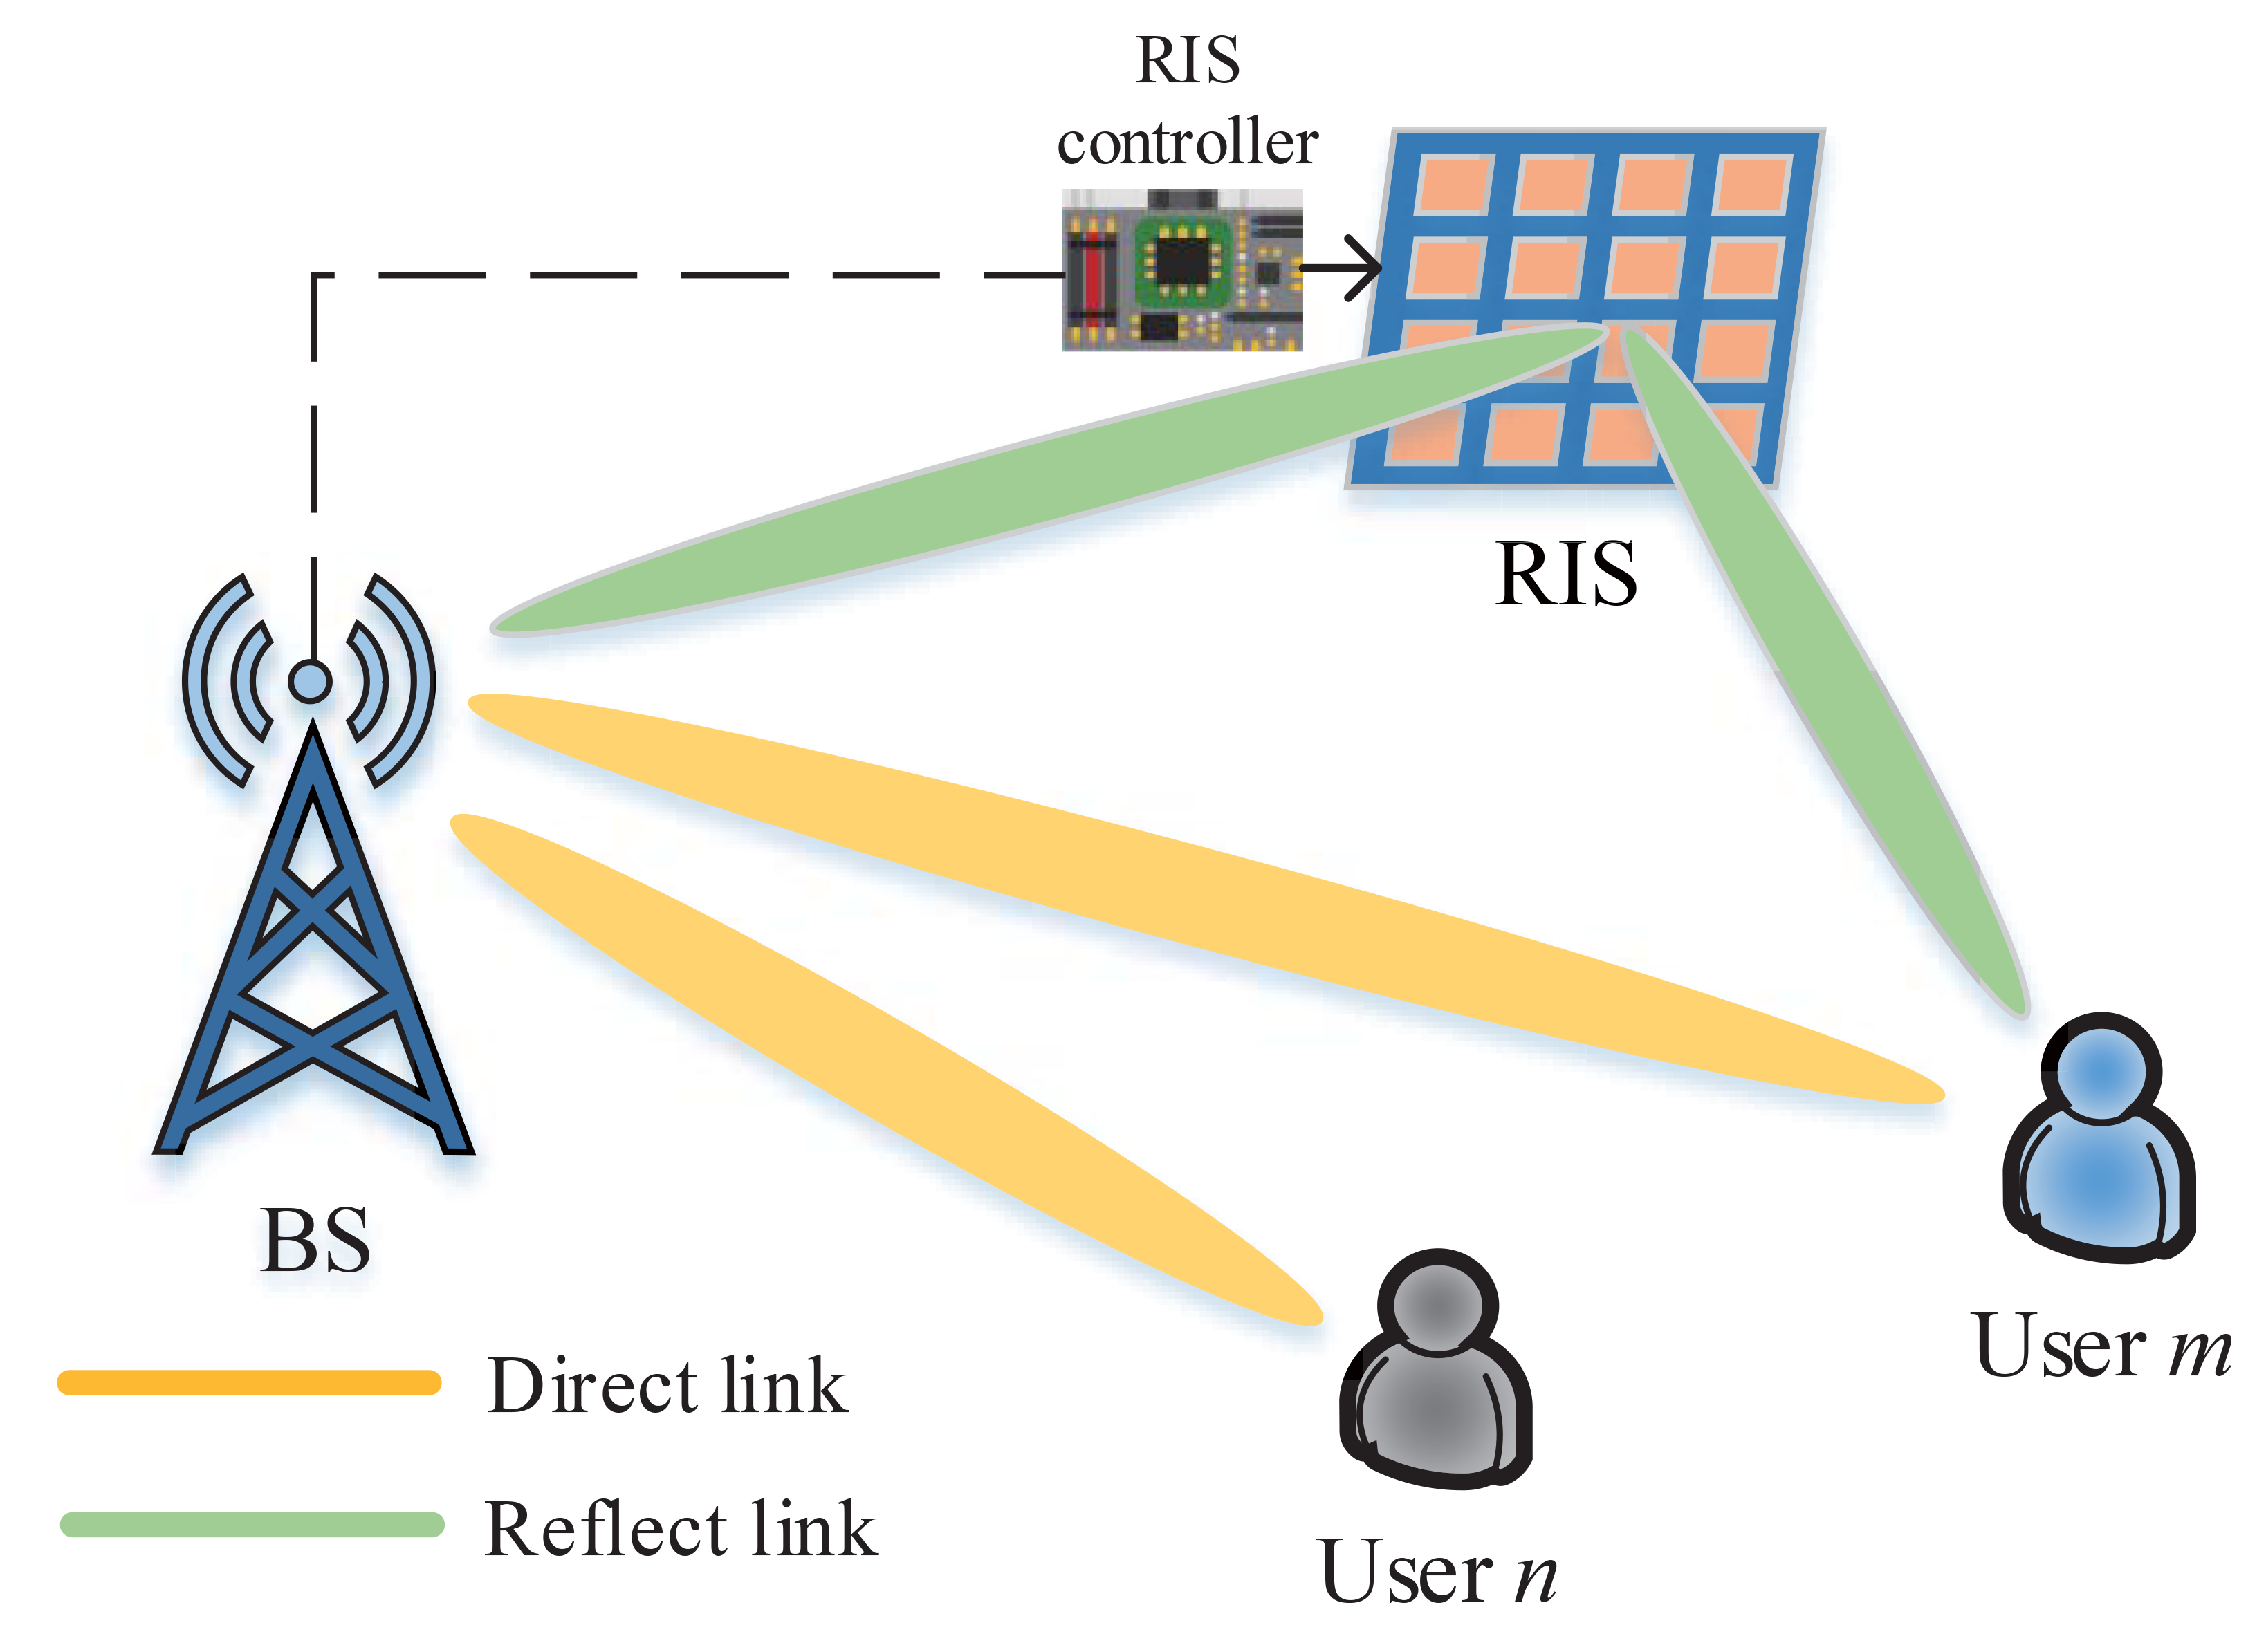
\includegraphics[totalheight=3cm]{Fig4.png}
  \end{figure}

\end{frame}

%------------------------------------------------

\begin{frame}
  \frametitle{RIS-Assisted Joint RadCom Beamforming Design}

  \begin{itemize}
    \item Optimization Problem
      \begin{align*}
        \max_{\mathbf{P},\mathbf{R}_x,\mathbf{\Theta}} \rho&\sum_{k=1}^K \mu_k R_k(\mathbf{P},\mathbf{R}_x,\mathbf{\Theta}) + \mathbf{a}_1^H(\varphi_m)\mathbf{R}_x \mathbf{a}_1(\varphi_m) + \mathbf{a}_2^H(\varphi_m)\mathbf{P}\mathbf{P}^H\mathbf{a}_2(\varphi_m) \\ 
        \mathbf{s.t.} \quad  &\mathrm{diag}(\mathbf{R}_x) = \frac{P_r \mathbf{1}^{M_r \times 1}}{M_r} 
        \\ &\mathrm{Tr} (\mathbf{P}\mathbf{P}^H) \leq P_c 
        \\ &\mathbf{R}_x \succeq 0 
        \\ &|\theta_n| \leq 1,n=1,...,N 
      \end{align*}
    \item Block Coordinate Descent, WMMSE \footfullcite{5199574} \footfullcite{9200993}, Fractional Programming \footfullcite{8314727}
  \end{itemize}
  \begin{figure}
    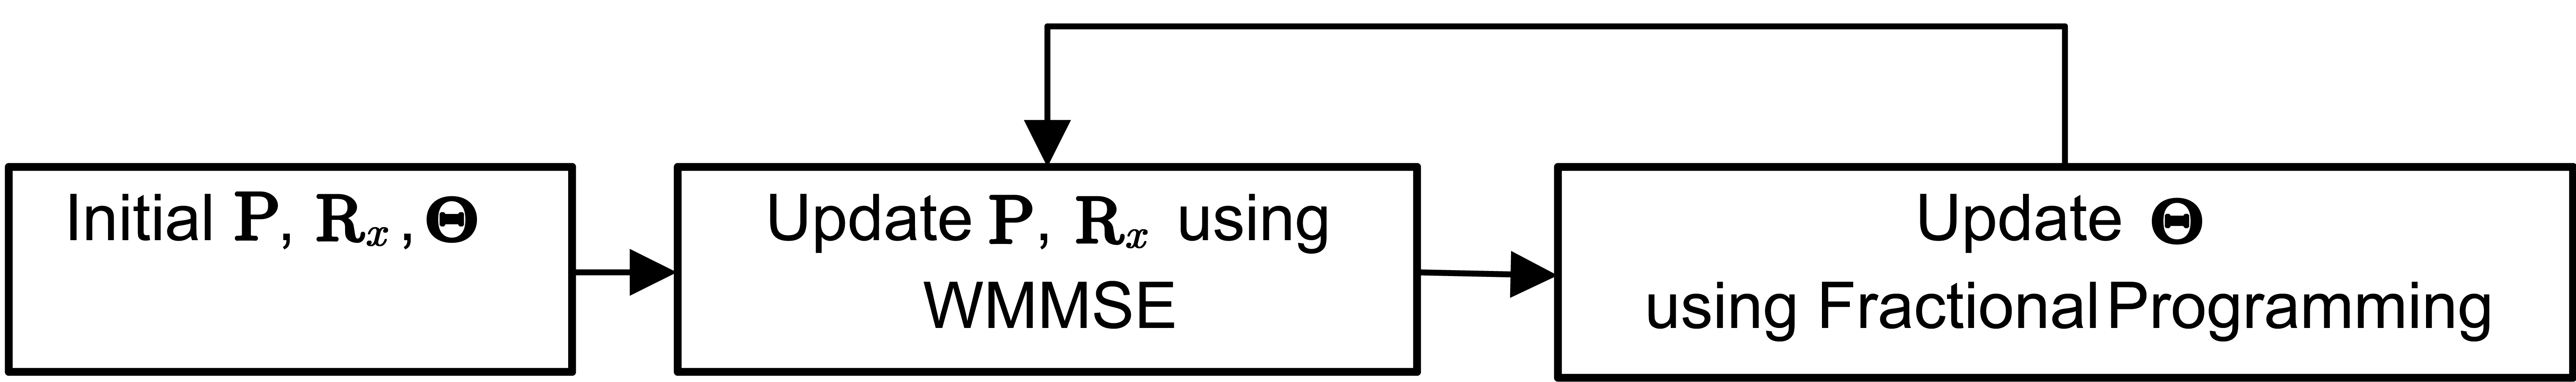
\includegraphics[width=0.9\linewidth]{Fig5.png}
  \end{figure}
\end{frame}

%------------------------------------------------

\begin{frame}
  \frametitle{RIS-Assisted Joint RadCom Beamforming Design}

  \begin{itemize}
    \item Update ${\mathbf{P}}$, ${\mathbf{R}}_x$ using WMMSE $\to$ Semi-definite Programming
      \begin{align*}
        \min_{\mathbf{P},\mathbf{R}_x} \rho&\sum_{k=1}^K \mu_k\xi_k(\mathbf{P},\mathbf{R}_x) - \mathbf{a}_1^H(\varphi_m)\mathbf{R}_x\mathbf{a}_1(\varphi_m) + \sum_{k=1}^K\mathbf{p}_k^H \mathbf{Z}(\varphi_m)\mathbf{p}_k
        \\ \mathbf{s.t.} \quad &\mathrm{diag}(\mathbf{R}_x) = \frac{P_r \mathbf{1}^{M_r \times 1}}{M_r} 
        \\ &\mathrm{Tr} (\mathbf{P}\mathbf{P}^H) \leq P_c 
        \\ &\mathbf{R}_x \succeq 0
      \end{align*}
    \item Update ${\mathbf{\Theta}}$ using Fractional Programming $\to$ Quadratic Programming 
      \begin{align*}
        \max_{\mathbf{y},\boldsymbol{\theta}} \sum_{k=1}^K&\left(2\mathfrak{R}\left\{y_k^*\sqrt{\tilde{\alpha}_k} \mathbf{a}_{k,k}^H \boldsymbol{\theta} \right\}-|y_k|^2\left(\sum_{j=1}^K|\mathbf{a}_{j,k}^H\boldsymbol{\theta} |^2 + \boldsymbol{\theta}^H \mathbf{B}_k \boldsymbol{\theta} + 1\right)\right) 
        \\  \mathbf{s.t.} \quad &|\theta_n| \leq 1,n=1,...,N 
        \\ &y_k \in \mathbb{C}
      \end{align*}
  \end{itemize}
\end{frame}

%------------------------------------------------

\begin{frame}
  \frametitle{RIS-Assisted Joint RadCom Beamforming Design}
  \begin{figure}
    
\includegraphics[width=1\linewidth]{Fig6.png}
  \end{figure}

\end{frame}

%------------------------------------------------

\begin{frame}
  \frametitle{Challenges}
  \begin{itemize}
    \item If the discrete phase shift of RIS is considered, the constraint set is non-convex
    \begin{itemize}
       \item Discrete set
    \end{itemize}
    \item If the shared deployment is considered, the constraint set is also  non-convex
    \begin{itemize}
      \item  Quadratic equality constraint
   \end{itemize}
  \end{itemize}

\end{frame}

%------------------------------------------------


\begin{frame}
\Huge{\centerline{Thanks}}
\end{frame}

%----------------------------------------------------------------------------------------

\end{document} 